\chapter{Traffic Safety Rule Engine}
\label{chap:safety}

\section{Overview}

The deterministic safety rule engine forms a central, priority-driven contribution of this project. Rather than treating safety assessment as an opaque black box, our framework formulates five independent, physics-grounded safety rules tailored to the complex dynamics of unsignalized roundabout traffic. Each rule encodes geometric, spatial, or kinematic conditions derived from physical road measurements and empirical traffic observations.

Section~\ref{sec:notation} establishes a unified mathematical notation system. Sections~\ref{sec:rule1} through \ref{sec:rule5} present the five safety rules in exact priority order: (i)~Unsafe Overtaking Detection, (ii)~Tailgating Detection, (iii)~Wrong-Way Driving Detection, (iv)~Erratic Lane Weaving Detection, and (v)~Vehicle Stoppage Detection. Each rule follows a standardized four-part structure: (i)~Intuition, (ii)~Algorithm, (iii)~Mathematical Model, and (iv)~Algorithmic Pseudocode.

\section{Unified Mathematical Notation}
\label{sec:notation}

All safety rules evaluate metric world-coordinate trajectories $(x_i(t), y_i(t))$ transformed into polar coordinates $(r_i(t), \theta_i(t))$ relative to the calibrated roundabout center $(X_C, Y_C) = (43.5, 28.5)$\,m:
\begin{equation}
    r_i(t) = \sqrt{(x_i(t) - X_C)^2 + (y_i(t) - Y_C)^2}, \qquad
    \theta_i(t) = \mathrm{atan2}(y_i(t) - Y_C,\;x_i(t) - X_C)
\end{equation}

Table~\ref{tab:notation} pre-explains the unified notation, state metrics, and threshold parameters used across all mathematical models and pseudocodes.

\begin{table}[H]
\centering
\small
\caption{Pre-explained mathematical notation and physical threshold system.}
\label{tab:notation}
\begin{tabularx}{\textwidth}{l X}
\toprule
\textbf{Symbol / Variable} & \textbf{Pre-Explained Definition / Physical Description} \\
\midrule
$i, j$ & Persistent vehicle track indices ($i = \text{evaluated vehicle}$, $j = \text{interacting target}$) \\
$t, f_{\text{ps}}$ & Video frame index $t$ at frame rate $f_{\text{ps}} = 30$ FPS \\
$(x_i(t), y_i(t))$ & World metric position coordinates of vehicle $i$ at frame $t$ (metres) \\
$r_i(t), \theta_i(t)$ & Polar radius (m) and polar angle (rad) of vehicle $i$ relative to $(X_C, Y_C)$ \\
$\mathrm{Lane}(r)$ & Lane assignment ($\text{Inner}: 6.0 \le r < 10.0$\,m, $\text{Outer}: 10.0 \le r \le 14.0$\,m) \\
$v_i(t), \omega_i(t)$ & Ground speed $v_i(t)$ (m/s) and angular velocity $\omega_i(t)$ (rad/s) \\
$d_{ij}(t)$ & Euclidean world distance between vehicles $i$ and $j$ (metres) \\
$d_{\text{arc\_ij}}(t)$ & Polar arc-length gap along curved lane center between follower $i$ and leader $j$ (m) \\
$\Delta_{ij}(t)$ & Signed relative polar angle difference $\mathrm{atan2}[\sin(\theta_j-\theta_i), \cos(\theta_j-\theta_i)]$ (rad) \\
$\Delta d_{90\_i}(t), \bar{v}_{90\_i}(t)$ & Retrospective 90-frame displacement (m) and rolling mean velocity (m/s) \\
\midrule
$D_{\text{overtake}}, \Delta R_{\text{max}}, V_{\text{min\_overtake}}$ & Overtaking thresholds ($D_{\text{overtake}} = 4.5$\,m, $\Delta R_{\text{max}} = 2.2$\,m, $V_{\text{min\_overtake}} = 0.8$\,m/s) \\
$D_{\text{tailgate}}, V_{\text{min\_tailgate}}$ & Tailgating thresholds ($D_{\text{tailgate}} = 4.0$\,m, $V_{\text{min\_tailgate}} = 1.0$\,m/s) \\
$\Omega_{\text{wrong}}, V_{\text{min\_wrong}}, N_{\text{wrong}}$ & Wrong-way thresholds ($\Omega_{\text{wrong}} = -0.1$\,rad/s, $V_{\text{min\_wrong}} = 1.5$\,m/s, $N_{\text{wrong}} = 45$) \\
$R_{\text{boundary}}, W_{\text{weaving}}, K_{\text{weaving}}$ & Weaving thresholds ($R_{\text{boundary}} = 10.0$\,m, $W_{\text{weaving}} = 90$, $K_{\text{weaving}} = 3$) \\
$D_{\text{stop}}, V_{\text{stop}}, W_{\text{stoppage}}$ & Stoppage thresholds ($D_{\text{stop}} = 1.0$\,m, $V_{\text{stop}} = 0.8$\,m/s, $W_{\text{stoppage}} = 90$) \\
\bottomrule
\end{tabularx}
\end{table}

% =========================================================================
\section{Rule 1: Unsafe Overtaking Detection}
\label{sec:rule1}

\subsection{Intuition}
Unsafe overtaking occurs when a passing vehicle executes a rapid, close-proximity passing maneuver around a target vehicle within the circulatory ring.

\subsection{Algorithm}
For each co-present pair $(i, j)$, the algorithm evaluates the relative polar angle difference $\Delta_{ij}(t)$. An overtaking action is identified when the sign of $\Delta_{ij}(t)$ flips between consecutive frames ($\Delta t \le 10$). An infraction is logged if Euclidean distance $d_{ij} \le D_{\text{overtake}} = 4.5$\,m, radial difference $|r_i - r_j| \le \Delta R_{\text{max}} = 2.2$\,m, and overtaker speed $v_i \ge V_{\text{min\_overtake}} = 0.8$\,m/s.

\subsection{Mathematical Model}
Signed relative polar angle difference:
\begin{equation}
    \Delta_{ij}(t) = \mathrm{atan2}\!\left[\sin(\theta_j(t)-\theta_i(t)),\;\cos(\theta_j(t)-\theta_i(t))\right]
\end{equation}
Sign-flip condition between frames $t_{\text{prev}}$ and $t$ ($t - t_{\text{prev}} \le 10$):
\begin{equation}
    \Delta_{ij}(t_{\text{prev}}) \cdot \Delta_{ij}(t) < 0 \quad\land\quad d_{ij}(t) \le D_{\text{overtake}}
\end{equation}
where $d_{ij}(t) = \sqrt{(x_i(t)-x_j(t))^2 + (y_i(t)-y_j(t))^2}$. The distance threshold $D_{\text{overtake}} = 4.5$\,m restricts detection to near-miss passing encounters.

\subsection{Pseudocode}
\begin{algorithm}[H]
\caption{Unsafe Overtaking Detection Algorithm}
\label{alg:rule1}
\begin{algorithmic}[1]
\Require Trajectories $\mathcal{T}$, parameters $D_{\text{overtake}} = 4.5$\,m, $\Delta R_{\text{max}} = 2.2$\,m, $V_{\text{min\_overtake}} = 0.8$\,m/s
\Ensure Unsafe overtaking records $\mathcal{V}_{\text{overtake}}$
\State $\mathcal{V}_{\text{overtake}} \gets \emptyset$
\For{each co-present vehicle pair $(i, j)$ in trajectories $\mathcal{T}$}
    \For{consecutive observations $t_{\text{prev}}, t$ with $t - t_{\text{prev}} \le 10$}
        \State Compute relative angle $\Delta_{ij}(t) \gets \mathrm{atan2}(\sin(\theta_j-\theta_i), \cos(\theta_j-\theta_i))$
        \If{$\Delta_{ij}(t_{\text{prev}}) \cdot \Delta_{ij}(t) < 0$}
            \State Compute distance $d_{ij}(t) \gets \sqrt{(x_i-x_j)^2 + (y_i-y_j)^2}$
            \If{$d_{ij}(t) \le D_{\text{overtake}}$ \textbf{and} $|r_i - r_j| \le \Delta R_{\text{max}}$ \textbf{and} $v_i \ge V_{\text{min\_overtake}}$}
                \State Record event $(t, \text{ID}_i, \text{ID}_j, d_{ij}, v_i)$ in $\mathcal{V}_{\text{overtake}}$
            \EndIf
        \EndIf
    \EndFor
\EndFor
\State \Return $\mathcal{V}_{\text{overtake}}$
\end{algorithmic}
\end{algorithm}

\subsection{Project Snapshot}
Figure~\ref{fig:unsafe_overtaking_plot} illustrates an unsafe overtaking event detected by Algorithm~\ref{alg:rule1} during trajectory evaluation.

\begin{figure}[H]
\centering
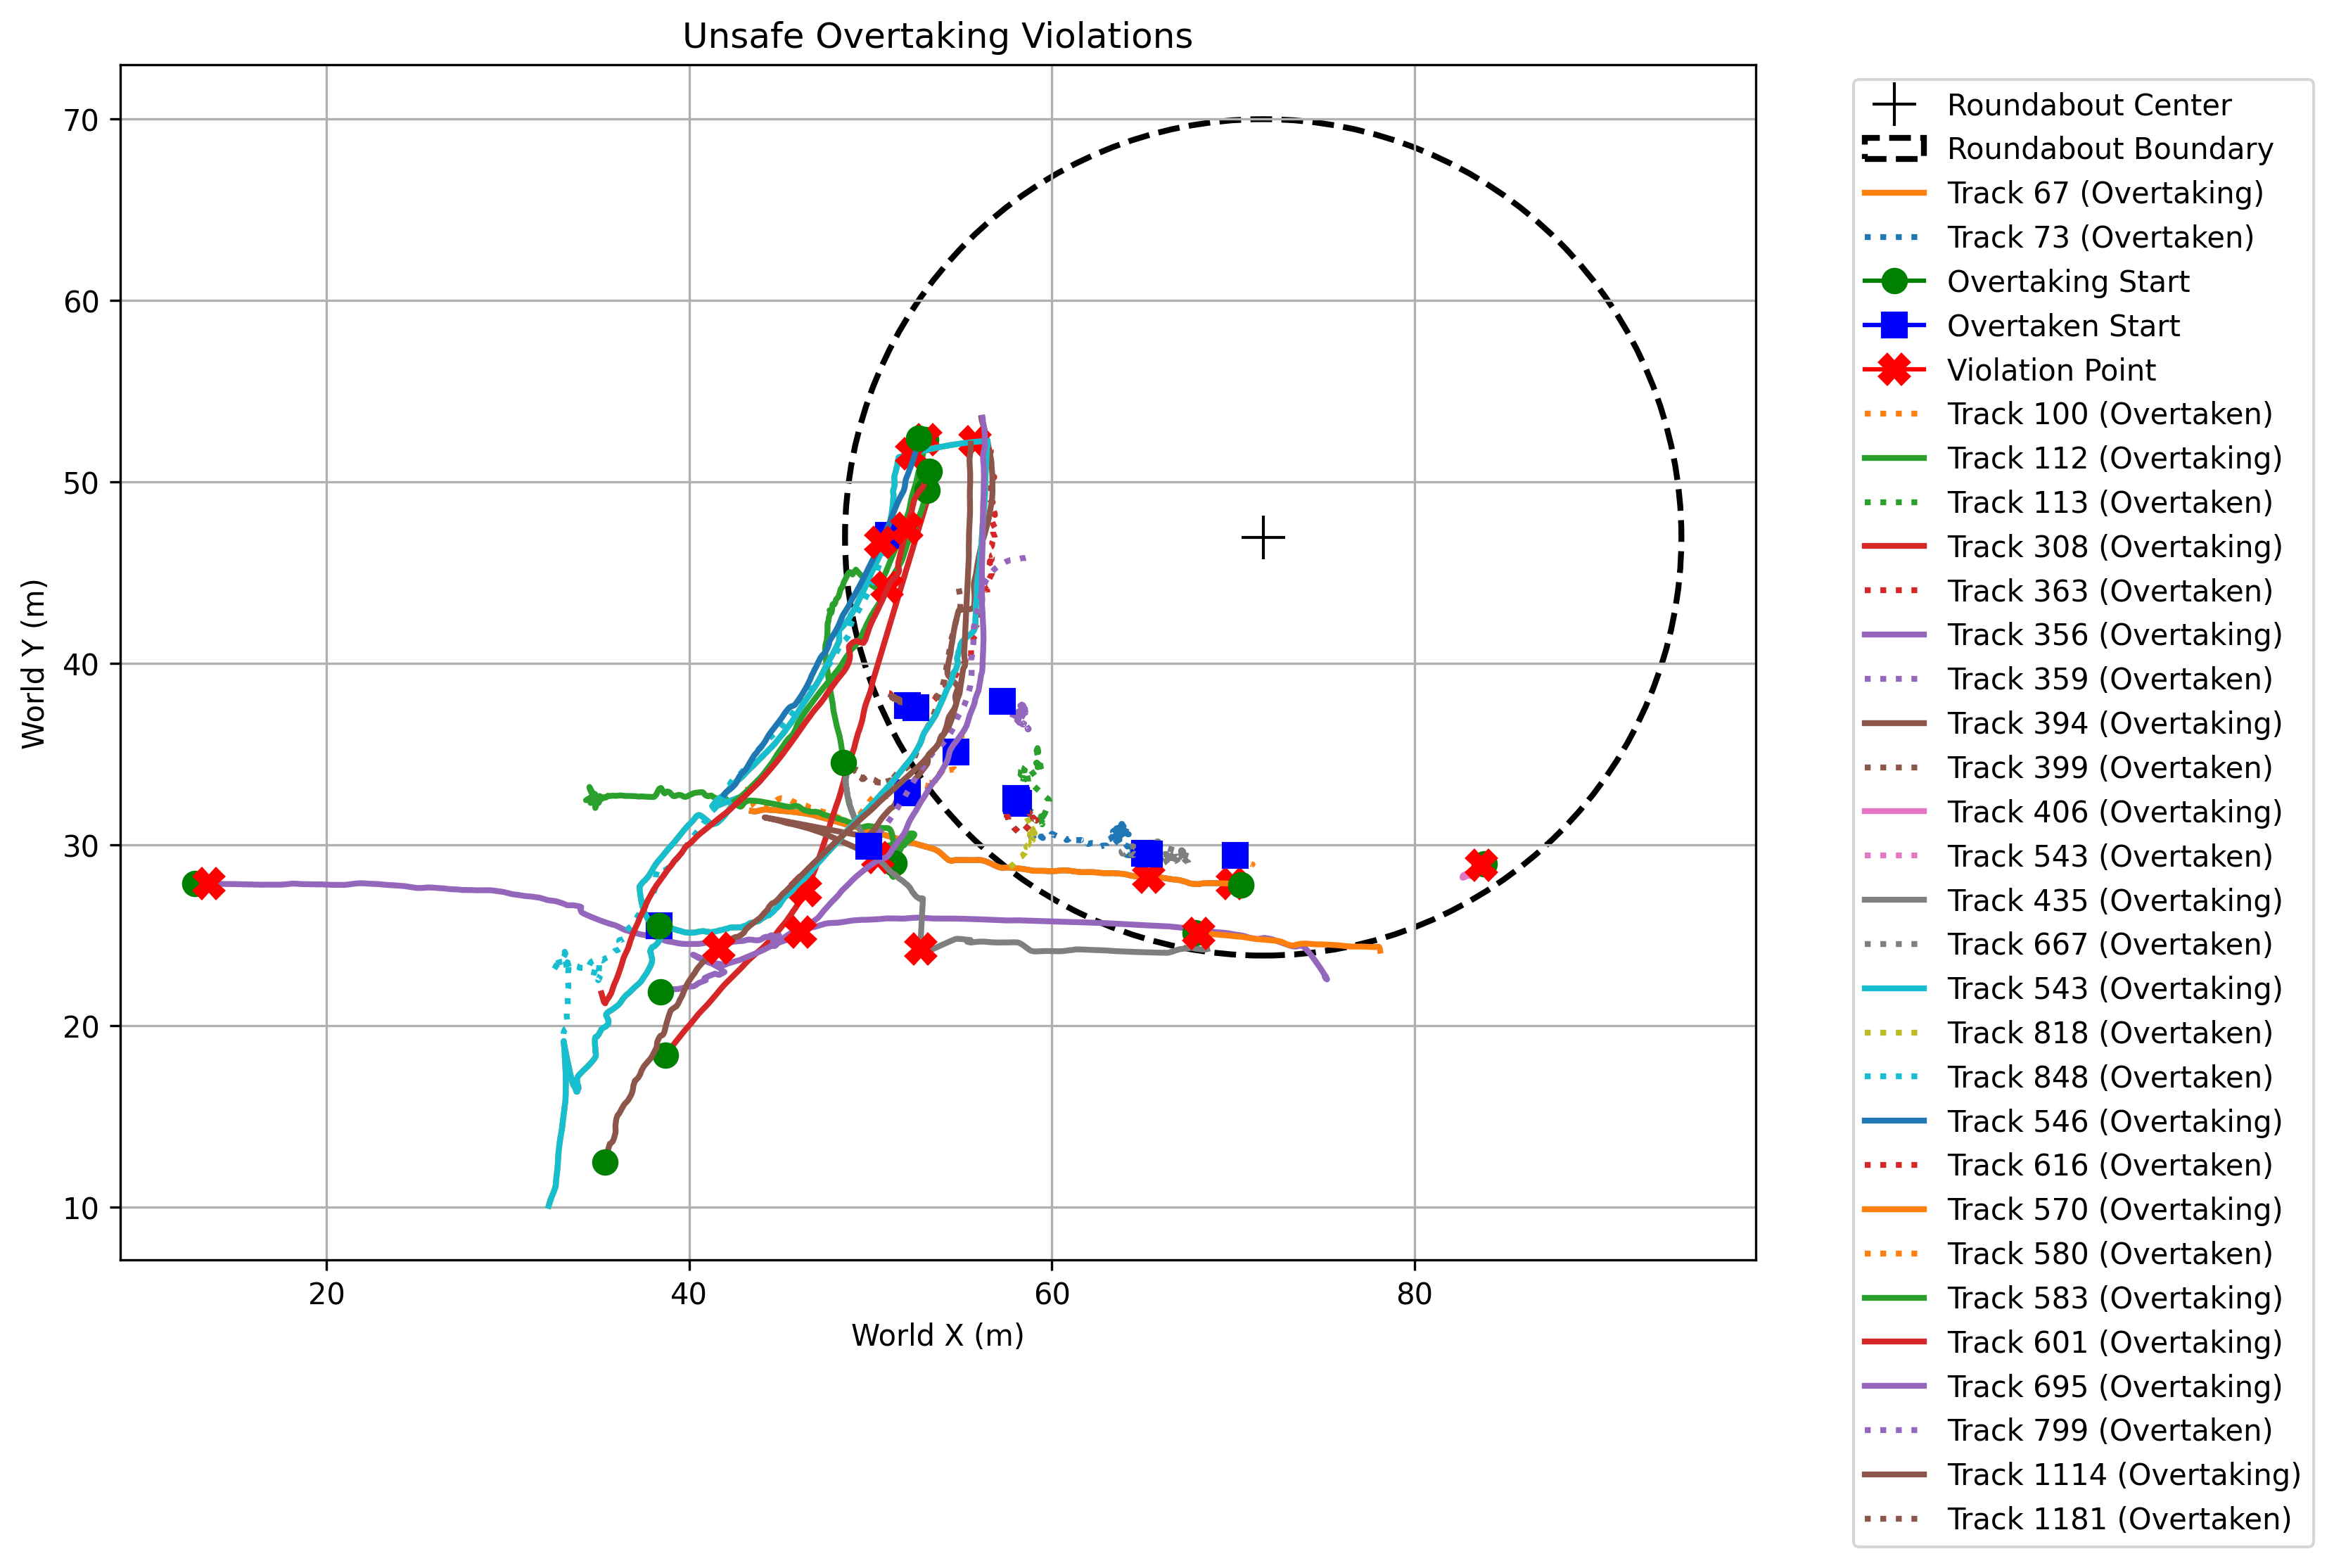
\includegraphics[width=0.55\textwidth]{../outputs/plots/overtaking.png}
\caption{Unsafe overtaking event identified by the safety rule framework. Trajectories of the overtaking vehicle (solid line) and overtaken vehicle (dotted line) are plotted alongside the exact violation trigger point (red marker).}
\label{fig:unsafe_overtaking_plot}
\end{figure}

% =========================================================================
\section{Rule 2: Tailgating Detection}
\label{sec:rule2}

\subsection{Intuition}
Tailgating occurs when a trailing follower vehicle follows a leading vehicle at an unsafe spatial gap while moving at active speed. In congested roundabout traffic, close following severely reduces reaction headway, elevating rear-end collision risk during sudden yields.

\subsection{Algorithm}
Vehicles within the same circulatory lane at frame $t$ are sorted by polar angle $\theta$. For consecutive follower--leader pairs $(i, j)$, the polar arc-length gap $d_{\text{arc\_ij}}$ is computed. A tailgating infraction is flagged if $d_{\text{arc\_ij}} < D_{\text{tailgate}} = 4.0$\,m and follower speed $v_i > V_{\text{min\_tailgate}} = 1.0$\,m/s.

\subsection{Mathematical Model}
The polar arc-length following distance along curved circulatory geometry is derived as:
\begin{equation}
    d_{\text{arc\_ij}}(t) = \left(\frac{r_i(t) + r_j(t)}{2}\right) \cdot \left[(\theta_j(t) - \theta_i(t)) \bmod 2\pi\right]
\end{equation}
where $r_i, \theta_i$ and $r_j, \theta_j$ denote the polar radii and angles of follower $i$ and leader $j$. The violation condition is:
\begin{equation}
    \mathcal{C}_{\text{tailgate}}(t) = \left( d_{\text{arc\_ij}}(t) < D_{\text{tailgate}} \right) \;\land\; \left( v_i(t) > V_{\text{min\_tailgate}} \right)
\end{equation}
The distance threshold $D_{\text{tailgate}} = 4.0$\,m corresponds to a 1.0-second headway at average roundabout speed ($\approx 4.0$\,m/s), while $v_i > 1.0$\,m/s prevents stationary queuing vehicles at entry points from triggering false positives.

\subsection{Pseudocode}
\begin{algorithm}[H]
\caption{Tailgating Detection Algorithm}
\label{alg:rule2}
\begin{algorithmic}[1]
\Require Trajectories $\mathcal{T}$, parameters $D_{\text{tailgate}} = 4.0$\,m, $V_{\text{min\_tailgate}} = 1.0$\,m/s
\Ensure Tailgating violation records $\mathcal{V}_{\text{tailgate}}$
\State $\mathcal{V}_{\text{tailgate}} \gets \emptyset$
\For{each frame $t$ and lane $L \in \{\text{Inner}, \text{Outer}\}$}
    \State Sort active vehicles in lane $L$ by ascending polar angle $\theta$
    \For{consecutive follower--leader pair $(i, j)$}
        \State Compute polar arc distance $d_{\text{arc\_ij}} \gets \frac{r_i + r_j}{2} \cdot \left[(\theta_j - \theta_i) \bmod 2\pi\right]$
        \If{$d_{\text{arc\_ij}} < D_{\text{tailgate}}$ \textbf{and} $v_i > V_{\text{min\_tailgate}}$}
            \State Record event $(t, \text{ID}_i, \text{ID}_j, L, d_{\text{arc\_ij}}, v_i)$ in $\mathcal{V}_{\text{tailgate}}$
        \EndIf
    \EndFor
\EndFor
\State \Return $\mathcal{V}_{\text{tailgate}}$
\end{algorithmic}
\end{algorithm}

% =========================================================================
\section{Rule 3: Wrong-Way Driving Detection}
\label{sec:rule3}

\subsection{Intuition}
Wrong-way driving occurs when a vehicle travels clockwise (opposite to mandatory counter-clockwise flow) inside the circulatory ring, creating critical head-on collision hazards.

\subsection{Algorithm}
Instantaneous angular velocity $\omega_i(t)$ is computed using continuous directional derivatives. A wrong-way violation is declared when $\omega_i(t) < \Omega_{\text{wrong}} = -0.1$\,rad/s and $v_i(t) \ge V_{\text{min\_wrong}} = 1.5$\,m/s continuously for $N_{\text{wrong}} \ge 45$ frames ($\approx 1.5$\,s).

\subsection{Mathematical Model}
Angular velocity is calculated via $\mathrm{atan2}$ phase-difference wrapping:
\begin{equation}
    \omega_i(t) = \mathrm{atan2}\!\left[\sin(\theta_i(t)-\theta_i(t{-}1)),\;\cos(\theta_i(t)-\theta_i(t{-}1))\right] \cdot f_{\text{ps}}
\end{equation}
The violation criterion requires sustained counter-directional motion:
\begin{equation}
    \sum_{m=0}^{N_{\text{wrong}}-1} \mathbb{1}\left[ \omega_i(t-m) < \Omega_{\text{wrong}} \;\land\; v_i(t-m) \ge V_{\text{min\_wrong}} \right] = N_{\text{wrong}}
\end{equation}
The 45-frame persistence requirement eliminates transient tracking noise, parking adjustments, and short evasive swerves.

\subsection{Pseudocode}
\begin{algorithm}[H]
\caption{Wrong-Way Driving Detection Algorithm}
\label{alg:rule3}
\begin{algorithmic}[1]
\Require Trajectories $\mathcal{T}$, parameters $\Omega_{\text{wrong}} = -0.1$\,rad/s, $V_{\text{min\_wrong}} = 1.5$\,m/s, $N_{\text{wrong}} = 45$
\Ensure Wrong-way violation records $\mathcal{V}_{\text{wrong}}$
\State $\mathcal{V}_{\text{wrong}} \gets \emptyset$
\For{each vehicle track $i$ inside ring $r_i \in [6.0, 14.0]$\,m}
    \State Initialize persistence counter $c_i \gets 0$
    \For{consecutive frames $t$}
        \State Compute $\omega_i(t) \gets \mathrm{atan2}(\sin(\theta_i(t)-\theta_i(t-1)), \cos(\theta_i(t)-\theta_i(t-1))) \cdot f_{\text{ps}}$
        \If{$\omega_i(t) < \Omega_{\text{wrong}}$ \textbf{and} $v_i(t) \ge V_{\text{min\_wrong}}$}
            \State $c_i \gets c_i + 1$
            \If{$c_i = N_{\text{wrong}}$}
                \State Record violation $(i, \text{class}_i, t - N_{\text{wrong}} + 1, t)$ in $\mathcal{V}_{\text{wrong}}$
            \EndIf
        \Else
            \State $c_i \gets 0$
        \EndIf
    \EndFor
\EndFor
\State \Return $\mathcal{V}_{\text{wrong}}$
\end{algorithmic}
\end{algorithm}

% =========================================================================
\section{Rule 4: Erratic Lane Weaving Detection}
\label{sec:rule4}

\subsection{Intuition}
Erratic lane weaving occurs when a vehicle executes rapid, un-signaled lateral transitions between inner and outer circulatory rings, destabilizing surrounding traffic flow.

\subsection{Algorithm}
Binary lane state $s_i(t) = \mathbb{1}[r_i(t) \ge R_{\text{boundary}}]$ where $R_{\text{boundary}} = 10.0$\,m is tracked per frame. An infraction is recorded when $K_{\text{weaving}} \ge 3$ boundary transitions occur within a rolling window of $W_{\text{weaving}} = 90$ frames ($\approx 3.0$\,s).

\subsection{Mathematical Model}
Given transition event set $\mathcal{E}_i = \{ t \mid s_i(t) \neq s_i(t{-}1) \land r_i(t) \in [6.0, 14.0] \}$, rolling window transition count is:
\begin{equation}
    n_{\text{weaving\_i}}(t) = | \{ t' \in \mathcal{E}_i \mid t - W_{\text{weaving}} + 1 \le t' \le t \} |
\end{equation}
The violation condition is:
\begin{equation}
    \mathcal{C}_{\text{weaving}}(t) = \left( n_{\text{weaving\_i}}(t) \ge K_{\text{weaving}} \right)
\end{equation}
Three lane transitions within 3 seconds distinguish reckless multi-lane weaving from standard single lane changes.

\subsection{Pseudocode}
\begin{algorithm}[H]
\caption{Erratic Lane Weaving Detection Algorithm}
\label{alg:rule4}
\begin{algorithmic}[1]
\Require Trajectories $\mathcal{T}$, parameters $R_{\text{boundary}} = 10.0$\,m, $W_{\text{weaving}} = 90$, $K_{\text{weaving}} = 3$
\Ensure Erratic lane weaving records $\mathcal{V}_{\text{weaving}}$
\State $\mathcal{V}_{\text{weaving}} \gets \emptyset$
\For{each vehicle track $i$ in trajectories $\mathcal{T}$}
    \State Extract transition set $\mathcal{E}_i \gets \{t \mid \mathbb{1}[r_i(t) \ge R_{\text{boundary}}] \neq \mathbb{1}[r_i(t-1) \ge R_{\text{boundary}}]\}$
    \For{each frame $t$}
        \State Compute window count $n_{\text{trans}} \gets |\{t' \in \mathcal{E}_i \mid t - W_{\text{weaving}} + 1 \le t' \le t\}|$
        \If{$n_{\text{trans}} \ge K_{\text{weaving}}$}
            \State Record event $(i, \text{class}_i, t - W_{\text{weaving}} + 1, t, n_{\text{trans}})$ in $\mathcal{V}_{\text{weaving}}$
        \EndIf
    \EndFor
\EndFor
\State \Return $\mathcal{V}_{\text{weaving}}$
\end{algorithmic}
\end{algorithm}

% =========================================================================
\section{Rule 5: Vehicle Stoppage Detection}
\label{sec:rule5}

\subsection{Intuition}
Vehicle stoppage occurs when a vehicle comes to an unauthorized complete stop inside an active circulatory lane, creating blockages for trailing traffic.

\subsection{Algorithm}
Deduplicated vehicle tracks ($d \ge 1.8$\,m / IoU $\le 0.20$) inside the circulatory ring are evaluated over a 90-frame retrospective window ($W_{\text{stoppage}} = 90$). A stoppage infraction is flagged when 90-frame displacement $\Delta d_{90\_i}(t) < D_{\text{stop}} = 1.0$\,m and rolling mean speed $\bar{v}_{90\_i}(t) < V_{\text{stop}} = 0.8$\,m/s.

\subsection{Mathematical Model}
Retrospective displacement and rolling mean velocity over window $W_{\text{stoppage}} = 90$ frames:
\begin{equation}
    \Delta d_{90\_i}(t) = \sqrt{(x_i(t)-x_i(t{-}90))^2 + (y_i(t)-y_i(t{-}90))^2}, \qquad
    \bar{v}_{90\_i}(t) = \frac{1}{90}\sum_{m=0}^{89} v_i(t-m)
\end{equation}
The violation condition is:
\begin{equation}
    \mathcal{C}_{\text{stoppage}}(t) = \left( \Delta d_{90\_i}(t) < D_{\text{stop}} \right) \;\land\; \left( \bar{v}_{90\_i}(t) < V_{\text{stop}} \right)
\end{equation}
Evaluating displacement over 3.0 seconds distinguishes prolonged vehicular blockages from temporary speed dips during yielding.

\subsection{Pseudocode}
\begin{algorithm}[H]
\caption{Vehicle Stoppage Detection Algorithm}
\label{alg:rule5}
\begin{algorithmic}[1]
\Require Trajectories $\mathcal{T}$, parameters $W_{\text{stoppage}} = 90$, $D_{\text{stop}} = 1.0$\,m, $V_{\text{stop}} = 0.8$\,m/s
\Ensure Vehicle stoppage records $\mathcal{V}_{\text{stop}}$
\State Apply deduplication filter on $\mathcal{T}$
\State $\mathcal{V}_{\text{stop}} \gets \emptyset$
\For{each vehicle track $i$ inside ring $r_i \in [6.0, 14.0]$\,m with duration $\ge W_{\text{stoppage}}$}
    \For{frame $t \ge W_{\text{stoppage}} - 1$}
        \State Compute $\Delta d_{90} \gets \sqrt{(x_i(t)-x_i(t-90))^2 + (y_i(t)-y_i(t-90))^2}$
        \State Compute $\bar{v}_{90} \gets \frac{1}{90}\sum_{m=0}^{89} v_i(t-m)$
        \If{$\Delta d_{90} < D_{\text{stop}}$ \textbf{and} $\bar{v}_{90} < V_{\text{stop}}$}
            \State Record event $(t, i, \mathrm{Lane}(r_i(t)), \Delta d_{90}, \bar{v}_{90})$ in $\mathcal{V}_{\text{stop}}$
        \EndIf
    \EndFor
\EndFor
\State \Return $\mathcal{V}_{\text{stop}}$
\end{algorithmic}
\end{algorithm}

\section{Rule Summary}

\begin{table}[H]
\centering
\small
\caption{Summary of safety rule conditions and output records (in priority evaluation order).}
\label{tab:rule_params}
\begin{tabularx}{\textwidth}{l X X}
\toprule
\textbf{Rule} & \textbf{Key Conditions} & \textbf{Output Record Fields} \\
\midrule
1. Unsafe Overtaking & sign flip of $\Delta_{ij}$, $d_{ij} \le 4.5$ m, $v_i \ge 0.8$ m/s & frame, overtaker ID, target ID \\
2. Tailgating      & $d_{\text{arc\_ij}} < 4.0$ m, $v_i > 1.0$ m/s & frame, follower ID, leader ID, lane, arc-distance \\
3. Wrong-Way       & $\omega_i < -0.1$ rad/s for $\ge 45$ frames, $v_i \ge 1.5$ m/s & track, class, start frame \\
4. Erratic Weaving & $\ge 3$ lane transitions in 90 frames & track, class, flagged-frame range \\
5. Vehicle Stoppage & $\Delta d_{90\_i} < 1.0$ m AND $\bar{v}_{90\_i} < 0.8$ m/s & frame, track, lane, displacement \\
\bottomrule
\end{tabularx}
\end{table}

The rule violation records exported by this stage are subsequently combined with manual dangerous-event annotations to form the ML training dataset (Chapter~\ref{chap:ml}).